
%(BEGIN_QUESTION)
% Copyright 2007, Tony R. Kuphaldt, released under the Creative Commons Attribution License (v 1.0)
% This means you may do almost anything with this work of mine, so long as you give me proper credit

In this high-temperature safety shutdown system, fuel shuts off to the burner only if {\it both} high-temperature switches and shutoff valves properly function.  Both switches have the same trip point, and both solenoid valves work identically.  The dependability rating for each switch/valve set is 0.6, which means each one is known to properly shut off fuel flow in the event of a high-temperature condition 60\% of the time:

$$\includegraphics[width=15.5cm]{i03599x01.eps}$$

A technician decides to calculate the probability of this system failing on demand.  That is, he intends to calculate how likely it will be that gas could continue to flow to the furnace even when the temperature was too high.  This is the technician's work to solve the problem:

$$
\includegraphics[width=15.5cm]{i03599x02.eps}$$

Identify both what is correct and what is incorrect in this technician's analysis of the system.

\vskip 10pt

\underbar{file i03599}
%(END_QUESTION)





%(BEGIN_ANSWER)

The technician was correct to apply the logical {\tt OR} function here: the system will fail to protect against high temperature if either switch/valve set A {\it or} switch/valve set B fails.  However, this is an {\it inclusive} {\tt OR} function rather than exclusive, which means the proper equation to use is:

$$P = A + B - AB$$

$$P = 0.4 + 0.4 - (0.16)$$

$$P = 0.64$$

\vskip 10pt

Another way to solve this is to calculate based on {\it dependability} rather than PFD.  We can say that the system requires both switch/valve set A {\it and} switch/valve set B to function properly in order for the shutdown system to shut the furnace down.  Thus:

$$
\includegraphics[width=15.5cm]{i03599x03.eps}$$


%(END_ANSWER)





%(BEGIN_NOTES)


%INDEX% Safety, system reliability: probability of failure on demand (PFD)

%(END_NOTES)


